\section{Optimization}%
\label{sec:optimization}
\subsection{Constraints}%
\label{sub:constraints}
How do you minimize the function stated above? First of all, you can let all of the confidences be equal to $0$, that way the loss function will be equal to $0$. This behavior should be invalid, and hence it is addressed in \ref{ssub:sinkhorn_knopp_algorithm}. What about negative confidences? That way, the losses that result might be negative. Implications are discussed within \ref{ssub:non_negative_matrices}.

\subsubsection{PLEASE Ignore this section}%
%\subsubsection{Sinkhorn-Knopp Algorithm}%
\label{ssub:sinkhorn_knopp_algorithm}
After I ran some tests, I realized that this approach didn't work as well as I thought it would. Please look at the next subsection.

Notice the characteristics of \autoref{fig:superpositionShade}. The sum of its confidences within its rows and columns are all equal to $1$. If the sum of the rows were not equal to 1, the probability of being within certain positions, would not be equal 1. And if the columns were not equal to one, that would mean that the probability of having certain token values would not equal to 1. The necessity for this constraint is reflected within the loss function itself. The loss could be zero if the confidences were zero. But this should be impossible, because there exists comparisons between tokens with non-zero values. So these constraints must be enforced.

A matrix that satisfies these constraints (rows and columns summing to one), is called a \emph{doubly stochastic matrix}. A well-known algorithm to convert any non-negative matrix into a doubly stochastic matrix is called the Sinkhorn-Knopp algorithm (also called RAS).\cite{sinkhorn1967concerning} There is a proof\cite{borobia1998matrix} and several papers\cite{chakrabarty2018better,knight2008sinkhorn} analyzing its convergence. Nonetheless, the algorithm itself is simple: iteratively normalizing the rows and columns of a matrix.

 Let $K$ be an $n\times n$ non-negative matrix. A single iteration of RAS is defined as follows:

\begin{align*}
        K'=&\begin{bmatrix}
                (\Sigma_j^N K_{1,j})^{-1}\\
                &\ddots{}\\
                &&(\Sigma_j^N K_{N,j})^{-1}
        \end{bmatrix}K &&\text{normalizing rows}\\
                K''=K'&\begin{bmatrix}
                (\Sigma_i^N K'_{i,1})^{-1}\\
                &\ddots{}\\
                &&(\Sigma_i^N K'_{i,N})^{-1}
        \end{bmatrix}&&\text{normalizing columns}
\end{align*}
Blank entries are $0$s. Here, normalizing rows simply means dividing each element by the sum of its row, and normalizing columns simply means dividing each element by the sum of its column. \autoref{fig:ras_demo} demonstrates the effectiveness of RAS. Graphed on the y-axis is the squared error, defined as:
\begin{align*}
        E(X)=\sum^N_i\left(\left(\sum^N_jX_{ij}\right)-1\right)^2+\sum^N_j\left(\left(\sum^N_iX_{ij}\right)-1\right)^2
\end{align*}
Although this does not prove the convergence of RAS, it at least demonstrates its effectiveness.

\begin{figure}[htpb]
        \centering
        % This file was created by tikzplotlib v0.9.1.
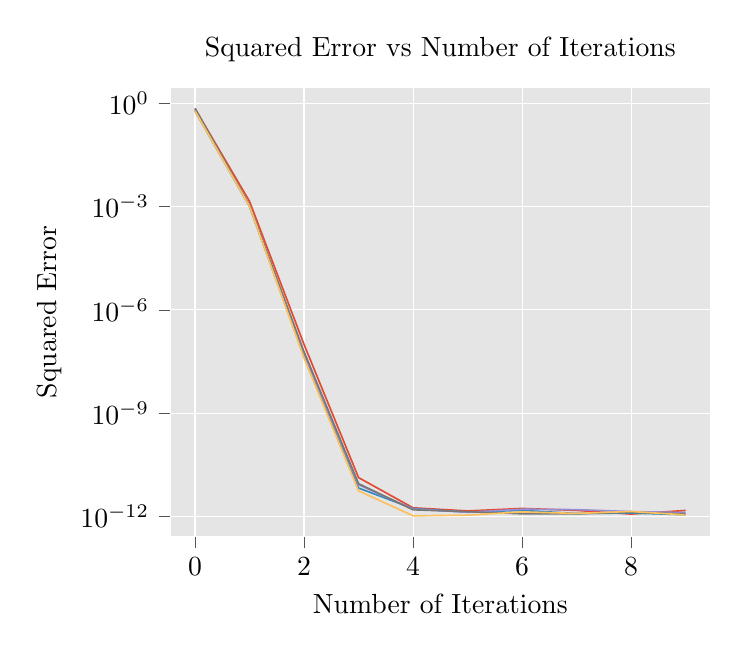
\begin{tikzpicture}

\definecolor{color0}{rgb}{0.886274509803922,0.290196078431373,0.2}
\definecolor{color1}{rgb}{0.203921568627451,0.541176470588235,0.741176470588235}
\definecolor{color2}{rgb}{0.596078431372549,0.556862745098039,0.835294117647059}
\definecolor{color3}{rgb}{0.984313725490196,0.756862745098039,0.368627450980392}

\begin{axis}[
axis background/.style={fill=white!89.8039215686275!black},
axis line style={white},
log basis y={10},
tick align=outside,
tick pos=left,
title={Squared Error vs Number of Iterations},
x grid style={white},
xlabel={Number of Iterations},
xlabel near ticks,
xmajorgrids,
xmin=-0.45, xmax=9.45,
xtick style={color=white!33.3333333333333!black},
y grid style={white},
ylabel={Squared Error},
ylabel near ticks,
ymajorgrids,
ymin=2.71273553797183e-13, ymax=2.77667975831396,
ymode=log,
ytick style={color=white!33.3333333333333!black}
]
\addplot [semithick, color0]
table {%
0 0.691431879997253
1 0.00141645281109959
2 9.95126896441434e-08
3 1.36033406761271e-11
4 1.80833126250945e-12
5 1.46727074934461e-12
6 1.73372427525464e-12
7 1.52411416820541e-12
8 1.19015908239817e-12
9 1.51345602716901e-12
};
\addplot [semithick, color1]
table {%
0 0.591166257858276
1 0.0010115496115759
2 4.45605756738132e-08
3 6.77857769915136e-12
4 1.71951342053944e-12
5 1.35713662530179e-12
6 1.52411416820541e-12
7 1.23634436022257e-12
8 1.27897692436818e-12
9 1.13686837721616e-12
};
\addplot [semithick, color2]
table {%
0 0.625002205371857
1 0.00102552131284028
2 5.11129663038901e-08
3 8.41993141875719e-12
4 1.66622271535743e-12
5 1.34292577058659e-12
6 1.64490643328463e-12
7 1.60227386913903e-12
8 1.406874616805e-12
9 1.31450406115619e-12
};
\addplot [semithick, white!46.6666666666667!black]
table {%
0 0.711470305919647
1 0.00108080555219203
2 6.08989694228512e-08
3 9.08784159037168e-12
4 1.58451030074502e-12
5 1.3962164757686e-12
6 1.21147536447097e-12
7 1.21147536447097e-12
8 1.33937305690779e-12
9 1.20792265079217e-12
};
\addplot [semithick, color3]
table {%
0 0.590315997600555
1 0.00102019123733044
2 3.97954451614169e-08
3 5.62394575354119e-12
4 1.05870867628255e-12
5 1.10844666778576e-12
6 1.37845290737459e-12
7 1.24344978758018e-12
8 1.4175327578414e-12
9 1.12265752250096e-12
};
\end{axis}

\end{tikzpicture}

        \caption{Demonstration of RAS convergence: 5 samples with $N=100$, randomly generated from a uniform distribution $[0,\frac{2}{N})$. Error is equal to the sum of squared errors of the sums of the rows and columns from 1. Note the logarithmic scale.}%
        \label{fig:ras_demo}
\end{figure}


\subsubsection{Non-negative Matrices}%
\label{ssub:non_negative_matrices}

Both because Sinkhorn-Knopp requires a non-negative matrix and because negative probabilities do not make sense, we have to ensure that the entries within $S$ are above  $0$. To do that, we can simply take the absolute value of all the entries, before applying RAS.
\begin{equation}
K'_{ij}=|K_{ij}|
\end{equation}

\subsection{Gradient Descent}%
\label{sub:gradient_descent}
Gradient Descent is an algorithm to iteratively optimize a convex function, with knowledge of the derivative of the function with respect to all of the function parameters $\theta$. In the case of optimizing a loss function, steps must be taken in the direction opposite to the gradient, therefore, the equation is as follows
\begin{equation}
         \theta'=\theta-\alpha \frac{\delta}{\delta \theta}L(\theta)
\end{equation}
where $\alpha$ is a parameter determining how big of a change there is between iterations of gradient descent.

\subsubsection{Negative Standard Deviation}%
\label{ssub:negative_standard_deviation}
In order to encourage discreteness, we can encourage sparseness within the matrix. That is, we would like one value to be larger than the others, this will help the algorithm within \ref{sec:discretization}. A common known metric to measure the spread of the data is called the standard deviation, and the biased standard deviation\footnote{Used for simplicity} is defined as follows:
\begin{align*}
    \frac{\sum_i^N \left(x_i-\overline{x}\right)^2}{N}
\end{align*}
But we want to have the value to increase when the spread decreases, so instead, we can the loss is the negative of the standard deviation. But we do not want to measure the spread against the mean, but rather, against the maximum (we want a single large maximum) so we take the negative of the maximum deviation:
\begin{align*}
    -\frac{N}{\sum_i^N \left(x_i-\max{x}\right)^2}
\end{align*}

\subsubsection{Derivative Coming Soon}%
\label{ssub:derivative_coming_soon}

\subsubsection{Partial Derivative of Loss Function}%
\label{ssub:derivative_of_loss_function}
The derivative of a multi-variable function \wrt{} a single variable, is called a partial-derivative, and is denoted by $\frac{\delta}{\delta x}$ instead of $\frac{d}{dx}$. Since our goal is to update each of the paramaters within $S$, we need to find a matrix which contains partial derivatives of the loss funtion against all of the elements.\footnote{This is very similar to Jacobian matrices; except that the Jacobian takes the partial derivatives of a vector against a vector, but we are taking partial derivatives of a scalar against a matrix.} That is, we are trying to find:
 \begin{align*}
         \frac{\delta L(S)}{\delta S}= \begin{bmatrix}
                 \frac{\delta L(S)}{\delta S_{1,1}}&\cdots &\frac{\delta L(S)}{\delta S_{1,N^2}}\\
                 \vdots &\ddots &\vdots \\
                 \frac{\delta L(S)}{\delta S_{N^2,1}}&\cdots &\frac{\delta L(S)}{\delta S_{N^2,N^2}}\\
         \end{bmatrix}
\end{align*}

To do that, we need to find the general solution to the partial derivative: $ \frac{\delta L(S)}{\delta S_{i,j}}$. Recall that the loss function is defined as
\begin{align*}
    L(S)=\frac{1}{2}\sum_{a}^{N^2} \sum_{b}^{N^2} \sum_{c}^{N^2} \sum_{d}^{N^2} S_{a,b} S_{c,d} C(O)_{a,c}C(O)_{b,d}
\end{align*}
Recall that in partial derivatives, only the variable in question (ie. $S_{i,j}$) is treated as a variable, the rest are treated as constants. We can see that the term $S_{i,j}$ is included within the loss when $(a,b)=(i,j)$ or $(c,d)=(i,j)$ or both. The derivatives are as following:
\begin{align*}
        \bm{A}=\frac{\delta L(S)}{\delta S_{i,j}}&=\frac{\delta}{\delta S_{i,j}}\left(\frac{1}{2}\sum_{c}^{N^2} \sum_{d}^{N^2} S_{i,j} S_{c,d} C(O)_{i,c}C(O)_{j,d}\right)&\text{First case}\\
              &=\frac{1}{2}\sum_{c}^{N^2} \sum_{d}^{N^2} S_{c,d} C(O)_{i,c}C(O)_{j,d}&\\
        \bm{B}=\frac{\delta L(S)}{\delta S_{i,j}}&=\frac{\delta}{\delta S_{i,j}}\left(\frac{1}{2}\sum_{a}^{N^2} \sum_{b}^{N^2} S_{a,b} S_{i,j} C(O)_{a,i}C(O)_{b,j}\right)&\text{Second case}\\
              &=\frac{1}{2}\sum_{a}^{N^2} \sum_{b}^{N^2} S_{a,b} C(O)_{a,i}C(O)_{b,j}&\\
        \bm{C}=\frac{\delta L(S)}{\delta S_{i,j}}&=\frac{\delta}{\delta S_{i,j}}\left(\frac{1}{2}S_{a,b} S_{a,b} C(O)_{a,b}C(O)_{a,b}\right)&\text{Third case}\\
              &=\frac{1}{2}\sum_{a}^{N^2} \sum_{b}^{N^2} S_{a,b} C(O)_{a,a}C(O)_{b,b}&\\
              &=0&
\end{align*}
$\bm{C}$ is $0$ because of the comparisons of tokens against themselves. The partial derivative of $L(S)$ against $S_{i,j}$ is equal to $\bm{A}+\bm{B}-\bm{C}=\bm{A}+\bm{B}$, because $\bm{A}$ and $\bm{B}$ represent all the cases in which $S_{i,j}$ is part of the loss function. Now, we can optimize $S$ with the Gradient Descent:
\begin{align*}
        S_{i,j}'=S_{i,j}-\alpha \left(\bm{A}+\bm{B}\right)
\end{align*}

\subsection{Optimization Procedure}%
\label{sub:optimization_procedure}

\subsubsection{Multi-objective Loss Function}%
\label{ssub:multi_objective_loss_function}
Now, we are satisfying multiple objectives: the negative maximum deviation, and the toroidal grid loss too. We can scale these by the losses by arbitrary parameters $\beta$ and $\gamma$

With all of the steps above, we can now optimize $S$. The procedure used within this essay is as following:\footnote{The procedure is by no means optimal. The purpose of this essay is not to be optimal, but to provide insight on what is possible.}
\begin{enumerate}
    \item Randomly initialize $S$ from a Uniform Distribution (equal probabilities for all values) on the interval $[0,1)$
    \item Repeat until convergence
    \begin{enumerate}
    \item Sum the Negative Maximum Deviation of all the rows and columns, and the Grid loss
    \item Calculate the partial derivatives
    item Perform Gradient Descent
    \end{enumerate}
\end{enumerate}
